\section*{Bayesian point estimation}
\begin{frame}{The maximum~\textit{a posteriori} (MAP) estimator}
\begin{defn}[Maximum~\textit{a posteriori}]
The posterior mode or maximum~\textit{a posteriori} (MAP) estimator of a parameter $\theta$ is given by
\begin{equation}
 \label{eq:MAP}
 \delta_{\pi}^{\text{MAP}}(x) := \argmax_{\theta \in \boldsymbol{\Theta}} p(\theta \mid x).
\end{equation}
\end{defn}
\begin{example}[MAP for the binomial case]
 Suppose $x \sim \operatorname{Binomial}(n, p)$.
 Now consider the following three priors for $p$: 
 \begin{itemize}
  \item $\pi_0(p) = \frac{\sqrt{p(1-p)}}{B(1/2, 1/2)} $ [Jeffreys];
  \item $\pi_1(p) = 1$ [Beta(1,1)/Uniform];
  \item $\pi_2(p) = \left(p(1-p)\right)^{-1}$ [\cite{Haldane1932}].  
 \end{itemize}
These lead to 
\begin{itemize}
 \item $\delta_0^{\text{MAP}}(x) = \max \{(x-1/2)/(n-1), 0 \}$;
 \item $\delta_1^{\text{MAP}}(x) = x/n$;
 \item $\delta_2^{\text{MAP}}(x) = \max \{ (x-1)/(n-2), 0 \}$.
\end{itemize}
\end{example}
\end{frame}
%%%%%%%%%%%%%%%%%%%%%%%%%%%%%%%%%%%
\begin{frame}{A word of caution}
 We end this discussion with the following warning:
\begin{idea}[Marginalise, not maximise]
\label{idea:always_marginalise}~
 Bayesian approaches to estimation and prediction \underline{usually} focus on \textit{marginalisation} rather than \textit{optmisation}.
 This is because, following the Likelihood Principle, all of the information available about the unknowns is contained in the posterior distribution, and thus all inferences must be made using this probability measure, usually by finding suitable expectations of functionals of interest.
\end{idea}
In particular, for higher dimensions, \textbf{concentration of measure}\footnote{See these excellent notes by Terence Tao:\url{https://terrytao.wordpress.com/2010/01/03/254a-notes-1-concentration-of-measure/} .} ensures that the posterior mode has less and less relevance as a summary, at least so far as the barycentre of the distribution is concerned.
\end{frame}
%%%%%%%%%%%%%%%%%%%%%%%%%%%%%%%%%%%
\begin{frame}{Precision of Bayes estimators}
 A central quantity in the evaluation of Bayesian estimators is
 \begin{equation}
  \label{eq:bayes_risk}
  E_p\left[\left(\delta_\pi - h(\theta)\right)^2\right] = E_{\pi}\left[\left(\delta_\pi - h(\theta)\right)^2 \mid x \right]
 \end{equation}
for measurable $h$.
\begin{example}[Bayes versus frequentist risk]
 Take $x \sim \operatorname{Binomial}(n, \theta)$ with $n$ known and place a Jeffreys's prior on $\theta$.
 Consider the MLE: $\delta_1(x) = x/n$.
 It can be shown that:
 $$ E_\pi\left[\left(\delta_1 - \theta \right)^2 \mid x \right] = \left(\frac{x - n/2}{n(n+1)}\right)^2 +  \frac{(x + 1/2)(n - x + 1/2)}{(n + 1)^2(n+2)}.$$
 Moreover,
 $$\max_{\theta \in (0, 1)}  E_\pi\left[\left(\delta_1 - \theta\right)^2 \mid x \right] = [4(n+2)]^{-1},$$
 and
 $$ \max_{\theta \in (0, 1)} E_\theta \left[\left(\delta_1 - \theta\right)^2\right] = [4n]^{-1}.$$ 
\end{example}
\end{frame}
%%%%%%%%%%%%%%%%%%%%%%%%%%%%%%%%%%%
\begin{frame}{A brief aside about prediction}
 Prediction is an important inferential task and is somewhat related to the previous discussion on precision.
 Consider predicting a quantity $z$ \textbf{conditional} on data $x$.
 For that  we need $g(z \mid x, \theta)$, $f(x\mid \theta)$ and $\pi(\theta)$.
 Then,
 \begin{equation}
  \label{eq:general_predictive}
  g_\pi(z\mid x) = \int_{\boldsymbol{\Theta}} g(z\mid x, t) p(t \mid x)\,dt
 \end{equation}
encodes all of the information brought by the posterior about $z$.
A special case  is i.i.d prediction:
\begin{equation}
 \label{eq:posterior_predictive_data}
 g(\tilde{x} \mid x) = \int_{\boldsymbol{\Theta}} f(\tilde{x} \mid t) p(t \mid x)\,dt
\end{equation}
is the posterior predictive of the new data $\tilde{x}$.
\begin{idea}[Calibrated priors for prediction]
\label{idea:prediction_calibrated_priors}
The prior, $\pi$, can be constructed so as to minimise error in a prediction task. 
\end{idea}
\end{frame}
%%%%%%%%%%%%%%%%%%%%%%%%%%%%%%%%%%%
\begin{frame}{A neat trick}
Computing expectations all the time means we have to become familiar with a few tricks to facilitate obtaining approximate answers.
\begin{example}[Mixture representation of the Student-t]
Take $x \sim \operatorname{Normal}_p(\theta, \boldsymbol{I}_p)$ and put $\theta \sim \operatorname{Student-t}_p(\alpha, 0, \tau^2\boldsymbol{I}_p)$.
Then $p(\theta \mid x)$ does not have a closed-form normalising constant and computing the Bayes estimator under quadratic loss is a chore.
However, we can use the representation
\begin{align*}
 \theta \mid z &\sim \operatorname{Normal}_p(0, \tau^2z\boldsymbol{I}_p),\\
 z & \sim \operatorname{InverseGamma}(\alpha/2, \alpha/2),
\end{align*}
to get 
$$ \theta \mid x, z \sim  \operatorname{Normal}_p\left(\frac{x}{ 1+ \tau^2z}, \frac{\tau^2z}{ 1+ \tau^2z}\boldsymbol{I}_p\right) $$ 
Thus, the Bayes estimator $\delta_\pi(x) = \int_0^\infty E_\pi[\theta \mid x, z]p(z \mid x)\,dz$ can be computed with a single integral for any dimension $p$. 
\end{example} 
\end{frame}
%%%%%%%%%%%%%%%%%%%%%%%%%%%%%%%%%%%
\begin{frame}{Conjugacy is handy!\footnote{Taken from~\cite{Robert2007}.}}
\begin{center}
 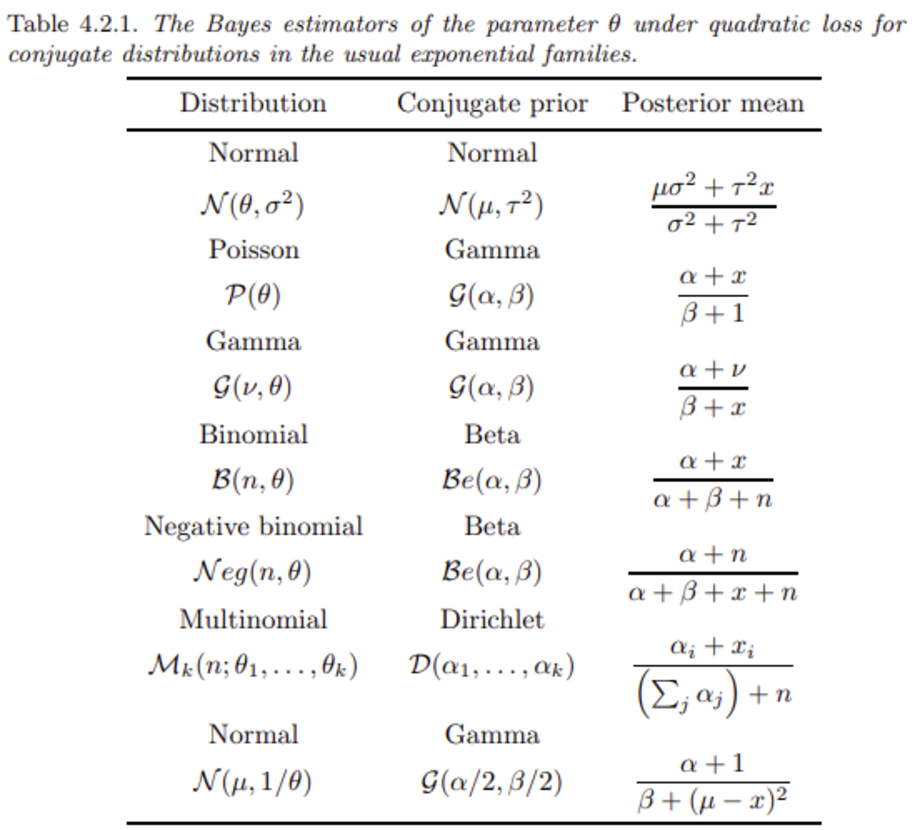
\includegraphics[scale=0.5]{figures/conjugate_table_expectations.pdf}
\end{center}
\end{frame}
%%%%%%%%%%%%%%%%%%%%%%%%%%%%%%%%%%%
\begin{frame}{A worked example}
We will stretch our Bayesian muscles with the next problem. 
\begin{exercise}[Inference for the rate of a Gamma]
\label{exercise:rate_gamma_different_losses}
 Let $x \sim \operatorname{Gamma}(\nu, \theta)$ with $\nu >0$ known.
 A natural choice of prior is $\theta \sim \operatorname{Gamma}(\alpha, \beta)$.
 Find the Bayes estimator under 
 $$ L_1(\delta, \theta) = \left(\delta - \frac{1}{\theta}\right)^2, $$
 and the scale-invariant loss
 $$ L_2(\delta, \theta) = \theta^2 \left(\delta - \frac{1}{\theta}\right)^2$$
 \textit{Hint:} If $X \sim \operatorname{Gamma}(\alpha, \beta)$, $Y = 1/X \sim \operatorname{InverseGamma}(\alpha, \beta)$ and $E[Y^k] = \frac{\beta^k}{(\alpha-1)\cdots(\alpha-k)}$
\end{exercise}
\end{frame}
%%%%%%%%%%%%%%%%%%%%%%%%%%%%%%%%%%%
\begin{frame}{A quick note on quadratic loss}
 Exercise~\ref{exercise:rate_gamma_different_losses} is a special case of the general situation where 
 $$ L(\delta, \theta) = w(\theta) ||\delta-\theta||_{\boldsymbol{G}}^2, $$
 for $\boldsymbol{G}$ a $p \times p$ non-negative symmetric matrix.
 In this case, we get
 $$ \delta_\pi = \frac{E_p[w(\theta)\theta]}{E_p[w(\theta)]}. $$
 Please \textbf{note} that there is no universal justification for quadratic loss other than (sometimes leading to increased) mathematical tractability
\end{frame}
%%%%%%%%%%%%%%%%%%%%%%%%%%%%%%%%%%%
\begin{frame}{Loss estimation}
 Since the loss function, $L(\delta(x), \theta)$ is usually measurable w.r.t the posterior, it can be estimated much the same way as other functionals.
 In particular, if you are feeling particularly eclectic, you can always constructed $\pi$ such that
 $$ E\left[E_p[L(\delta_\pi(x), \theta]\right] \geq R(\delta_\pi(x), \theta),  \theta \in \boldsymbol{\Theta}, $$
 i.e. that the estimated loss never underestimates the error resulting from the use of $\delta_\pi$, at least in the long run.
 This is called \textbf{frequentist validity}.
 \end{frame}
%%%%%%%%%%%%%%%%%%%%%%%%%%%%%%%%%%%
\begin{frame}{A nice little problem by Neyman}
The following problem is described by Jeffreys as originating with Jerzy Neyman\footnote{Jerzy Neyman (1894-1981) was a Polish-American statistician, known for with work with Egon Pearson (1895-1980) on the foundations of the null hypothesis significance testing (NHST) framework.}.
\begin{exercise}[The tramcar problem]
 \label{exercise:tramcar}
 A person travelling in a a foreign country has to change trains at a junction, and goes into the town, the existence of which they have only just heard.
 They have no idea of its size.
 The first thing they see is a tramcar numbered $100$.
 Assuming tramcars are numbered consecutively from $1$ onwards, what could one \textit{infer} about the number $N$ of tramcars in this town?
\end{exercise}
\end{frame}

%%%%%%%%%%%%%%%%%%%%%%%%%%%%%%%%%%%
\begin{frame}{Recommended reading}
\begin{itemize}
  \item[\faBook] \cite{Robert2007}, Ch4.
%  \item 
 \item[\faForward] Next lecture: \cite{Robert2007} Ch. 5.
 \end{itemize} 
\end{frame}
